\chapter{认识硬件}
\section{一般台式机键盘}
一般台式机键盘见图~\ref{fig:1}。由于此年龄的家长通常会接触到手机和台式机,首先来介绍一下台式机的常用功能键。
\begin{figure}[htbp]
	\centering
	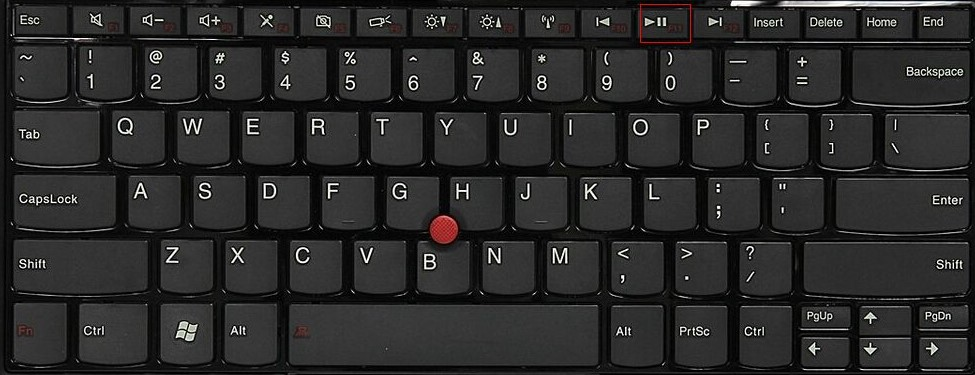
\includegraphics[width=0.7\linewidth]{figure/键盘}
	\caption{}
	\label{fig:1}
\end{figure}
\section[台式机常用功能键]{台式机常用功能键\footnotemark}
\footnotetext{以下顺序按照键盘上由上至下、由左至右的顺序,可直接对照自己键盘寻找}
\subsection{\seckeys{Esc} (退出键)}
\begin{description}
	\item [退出全屏]
	打开视频或者 PPT 的全屏时,若要退出全屏可直接按 \keys{Esc} 键退出
	\item [退出当前开启小界面]
	当点错某个网址,可以直接按 \keys{Esc} 键退出打开当前网页
	\item [清空表格]
	即清空当前编辑表格内的全部内容。
\end{description}

\subsection{\seckeys{Tab} (表格键)}
\begin{description}
	\item [缩进字符]
	当有很多空格需要打时,就使用 \keys{Tab} 键。
\end{description}
\subsection{\seckeys{Caps} (英文大小写切换)}
\subsection{\seckeys{Shift} (切换键)}
\begin{description}
	\item [一般 \keys{Ctrl + Shift} 键表示输入法循环并切换到所需要输入法(五笔,简体拼音,英文等)]
	\item [切换半角和全角%
	\footnote{半角简单来说就是英文字符,占一个空间的一半;全角就是中文字符,占满整个空间。}]
	\item [\keys{Delete + Shift} 不经过回收站直接删除文件]
	这种删除很难找回,建议误操作后找专人来清,当时不要选择重启或载入文件。
	\item [取消开机时启动其他附属软件]
	在开机界面出来后长按 \keys{Shift} 键,可以避免电脑隐藏软件的开机自启动。一般电脑里不经意安装的游戏或者附属软件,可以避免恶意开启占用网速。
\end{description}
\subsection{\seckeys{Ctrl} (控制键)}
不长篇赘述,之后会讲到组合键系列。
\subsection{\seckeys{Win} (菜单键)}
\begin{description}
	\item [打开开始菜单]
	\item [配合字母 \keys{E} 打开文件夹:\keys{Win+E}]
	\item [配合字母 \keys{D} 最小化所有窗口:\keys{Win+D}]
\end{description}
\subsection{\seckeys{Alt} (替换键)}
不长篇赘述,之后会讲到组合键系列
\subsection{\seckeys{Enter} (回车键)}
\begin{description}
	\item [换行]
	\item [确认当前所打内容]
\end{description}